\documentclass[11pt,a4paper]{article}

% Packages
\usepackage[utf8]{inputenc}
\usepackage[margin=1in]{geometry}
\usepackage{graphicx}
\usepackage{tabularx}
\usepackage{booktabs}
\usepackage{longtable}
\usepackage{xcolor}
\usepackage{colortbl}
\usepackage{fancyhdr}
\usepackage{titlesec}
\usepackage{hyperref}
\usepackage{enumitem}
\usepackage{tikz}
\usetikzlibrary{shapes.geometric,arrows.meta,positioning}
\usepackage{amsmath}
\usepackage{amssymb}  % Required for \checkmark
\usepackage{multirow}
\usepackage{array}
\usepackage{caption}
\usepackage{float}
\usepackage{pdflscape}
\usepackage{pifont}  % For additional symbols

% Color definitions
\definecolor{headerblue}{RGB}{0,102,204}
\definecolor{lightgray}{RGB}{240,240,240}
\definecolor{darkgray}{RGB}{100,100,100}
\definecolor{green}{RGB}{0,153,76}
\definecolor{red}{RGB}{204,0,0}
\definecolor{orange}{RGB}{255,140,0}

% Header and footer
\pagestyle{fancy}
\fancyhf{}
\fancyhead[L]{\small Career Assessment Platform - Hosting Analysis}
\fancyhead[R]{\small \today}
\fancyfoot[C]{\thepage}

% Title formatting
\titleformat{\section}
  {\Large\bfseries\color{headerblue}}
  {\thesection}{1em}{}[\titlerule]

\titleformat{\subsection}
  {\large\bfseries\color{headerblue}}
  {\thesubsection}{1em}{}

% Hyperref setup
\hypersetup{
    colorlinks=true,
    linkcolor=headerblue,
    filecolor=magenta,      
    urlcolor=blue,
    pdftitle={Hosting Comparison Report},
    pdfauthor={Technical Analysis},
}

% Custom commands - FIXED
\newcommand{\pro}{\textcolor{green}{\ding{51}}}  % Checkmark
\newcommand{\con}{\textcolor{red}{\ding{55}}}    % X mark
\newcommand{\neutral}{\textcolor{orange}{$\sim$}} % Tilde

\begin{document}

% Title page
\begin{titlepage}
    \centering
    \vspace*{2cm}
    
    {\Huge\bfseries Career Assessment Platform\par}
    \vspace{1cm}
    {\LARGE Hosting Infrastructure Comparison\par}
    \vspace{0.5cm}
    {\Large Dedicated Servers vs.  Managed Cloud Services\par}
    
    \vspace{2cm}
    
    {\large\itshape Comprehensive Technical \& Financial Analysis\par}
    
    \vfill
    
    % Application stack info
    \begin{tabular}{rl}
        \textbf{Backend: } & FastAPI (Python 3.x) \\
        \textbf{Frontend:} & React 19 + Vite \\
        \textbf{Database:} & SQLite → PostgreSQL/MySQL \\
        \textbf{Architecture:} & Monolithic API-driven \\
    \end{tabular}
    
    \vfill
    
    {\large \today\par}
\end{titlepage}

\tableofcontents
\newpage

% Executive Summary
\section{Executive Summary}

\subsection{Quick Decision Matrix}

\begin{table}[H]
\centering
\caption{Hosting Solution Comparison - Quick Reference}
\begin{tabularx}{\textwidth}{|l|X|X|}
\hline
\rowcolor{headerblue}
\textcolor{white}{\textbf{Criterion}} & \textcolor{white}{\textbf{Dedicated Servers}} & \textcolor{white}{\textbf{Managed Cloud}} \\
\hline
\textbf{Initial Cost (12mo)} & \$290-\$1,800 & \$180-\$4,800 \\
\hline
\textbf{Setup Time} & 2-5 days & 15 min - 2 hours \\
\hline
\textbf{DevOps Complexity} & High & Low-Medium \\
\hline
\textbf{Scalability} & Manual, Limited & Automatic, Unlimited \\
\hline
\textbf{Best For} & Predictable loads & Variable/growing loads \\
\hline
\textbf{Control Level} & Complete & Shared/Limited \\
\hline
\textbf{Uptime SLA} & 99.0-99.5\% & 99.9-99.99\% \\
\hline
\textbf{Performance} & Consistent & Variable \\
\hline
\rowcolor{lightgray}
\textbf{Recommended For Your App} & \textbf{Growth Phase} & \textbf{MVP \& Scale Phase} \\
\hline
\end{tabularx}
\end{table}

\subsection{Key Findings}

\begin{enumerate}[leftmargin=*]
    \item \textbf{For MVP/Startup Phase (<1,000 users):} Managed cloud platforms (Railway, Render, DigitalOcean App Platform) offer the fastest time-to-market with costs of \$5-\$60/month (verified 2026 pricing).
    
    \item \textbf{For Growth Phase (1K-10K users):} Dedicated servers become cost-effective at \$49-\$150/month, but require DevOps expertise.  Alternative:  DigitalOcean Droplets (\$24-\$96/month) or AWS Lightsail with managed database. 
    
    \item \textbf{For Scale Phase (>10K users):} Hybrid approach recommended:  Managed cloud for auto-scaling compute + dedicated database server.  Estimated \$300-\$800/month. 
    
    \item \textbf{CPU-Intensive Workload (PDF Generation):} Dedicated servers provide 30-40\% better performance-per-dollar for CPU-bound tasks like ReportLab + Matplotlib rendering.
    
    \item \textbf{Operational Complexity:} Managed cloud reduces operational overhead by 70-80\% but at 2-3x higher base costs for equivalent resources.
\end{enumerate}

\subsection{Strategic Recommendation}

\begin{table}[H]
\centering
\caption{Phase-Based Deployment Strategy (Updated 2026 Pricing)}
\begin{tabularx}{\textwidth}{|l|X|l|}
\hline
\rowcolor{headerblue}
\textcolor{white}{\textbf{Phase}} & \textcolor{white}{\textbf{Recommended Solution}} & \textcolor{white}{\textbf{Monthly Cost}} \\
\hline
\textbf{Phase 1: MVP} & Railway Hobby (\$5 plan + usage) or & \$5-\$50 \\
(0-1K users) & Render Free/Starter + PostgreSQL & \\
\hline
\textbf{Phase 2: Growth} & DigitalOcean Droplet (2-4 vCPU) + & \$84-\$150 \\
(1K-10K users) & Managed PostgreSQL, Docker deployment & \\
\hline
\textbf{Phase 3: Scale} & AWS/GCP Auto-scaling + RDS/Cloud SQL & \$300-\$800 \\
(10K+ users) & Multi-region, CDN, load balancing & \\
\hline
\end{tabularx}
\end{table}

\newpage

% Technical Fit Analysis
\section{Technical Fit Analysis}

\subsection{FastAPI + React Architecture Compatibility}

\begin{table}[H]
\centering
\caption{Platform Compatibility with Your Stack}
\small
\begin{tabularx}{\textwidth}{|l|X|X|}
\hline
\rowcolor{headerblue}
\textcolor{white}{\textbf{Platform}} & \textcolor{white}{\textbf{FastAPI Support}} & \textcolor{white}{\textbf{React/Vite Support}} \\
\hline
\textbf{Railway} & \pro Native (Nixpacks auto-detect) & \pro Static site deployment \\
\hline
\textbf{Render} & \pro Native ASGI support & \pro CDN-backed static sites \\
\hline
\textbf{Heroku} & \pro Gunicorn + Uvicorn workers & \pro Buildpack support \\
\hline
\textbf{AWS Lightsail} & \neutral Manual setup (Ubuntu + systemd) & \neutral S3 + CloudFront \\
\hline
\textbf{DigitalOcean} & \pro App Platform native & \pro Static site hosting \\
\hline
\textbf{Dedicated Server} & \pro Complete control (Nginx/systemd) & \pro Nginx static serving \\
\hline
\textbf{GCP Cloud Run} & \pro Container-native (auto-scaling) & \neutral Cloud Storage + CDN \\
\hline
\textbf{Azure App Service} & \pro Python 3.x runtime support & \pro Static Web Apps \\
\hline
\end{tabularx}
\end{table}

\subsection{Database Migration Path Analysis}

Your current SQLite database requires migration to PostgreSQL or MySQL for production. Here's the compatibility breakdown:

\begin{table}[H]
\centering
\caption{Database Service Options (2026 Verified Pricing)}
\begin{tabularx}{\textwidth}{|l|l|X|l|}
\hline
\rowcolor{headerblue}
\textcolor{white}{\textbf{Service}} & \textcolor{white}{\textbf{Type}} & \textcolor{white}{\textbf{Features}} & \textcolor{white}{\textbf{Price/mo}} \\
\hline
\textbf{AWS RDS PostgreSQL} & Managed & Auto-backups, read replicas, encryption & \$15-\$200 \\
\hline
\textbf{GCP Cloud SQL} & Managed & HA, point-in-time recovery, auto-scaling & \$10-\$180 \\
\hline
\textbf{Azure Database} & Managed & Zone redundancy, intelligent perf & \$12-\$190 \\
\hline
\textbf{DigitalOcean DB} & Managed & Simple pricing, auto-backups & \$15-\$120 \\
\hline
\textbf{Railway PostgreSQL} & Managed & Usage-based, generous free tier & \$0-\$50 \\
\hline
\textbf{Render PostgreSQL} & Managed & Free tier (30 days), auto-backups & \$0-\$95 \\
\hline
\textbf{Self-managed (VPS)} & Unmanaged & Full control, DIY backups & \$0 (included) \\
\hline
\end{tabularx}
\end{table}

\textbf{SQLAlchemy Migration Notes:}
\begin{itemize}
    \item Your existing SQLAlchemy ORM code requires minimal changes
    \item Change connection string from \texttt{sqlite:///database.db} to PostgreSQL format
    \item Update database URL in environment variables
    \item Use Alembic for schema migrations
    \item Test async SQLAlchemy with \texttt{asyncpg} driver
\end{itemize}

\subsection{CPU-Intensive PDF Generation Support}

Your ReportLab + Matplotlib workflow is CPU-bound (600 DPI rendering). Performance comparison:

\begin{table}[H]
\centering
\caption{PDF Generation Performance Estimates}
\begin{tabularx}{\textwidth}{|l|l|X|l|}
\hline
\rowcolor{headerblue}
\textcolor{white}{\textbf{Platform}} & \textcolor{white}{\textbf{vCPU}} & \textcolor{white}{\textbf{Est.  Render Time}} & \textcolor{white}{\textbf{Concurrent Jobs}} \\
\hline
\textbf{Dedicated (Ryzen 5)} & 4 cores & 2-3 seconds/report & 8-12 \\
\hline
\textbf{AWS t3.medium} & 2 vCPU & 4-6 seconds/report & 3-4 \\
\hline
\textbf{GCP e2-standard-2} & 2 vCPU & 4-5 seconds/report & 3-4 \\
\hline
\textbf{DigitalOcean 4GB} & 2 vCPU & 5-7 seconds/report & 2-3 \\
\hline
\textbf{Railway/Render Basic} & 1 vCPU & 8-12 seconds/report & 1-2 \\
\hline
\textbf{Heroku Standard} & 1 vCPU & 10-15 seconds/report & 1-2 \\
\hline
\end{tabularx}
\end{table}

\textbf{Optimization Recommendations:}
\begin{enumerate}
    \item Implement async task queue (Celery + Redis) for PDF generation
    \item Use background workers to prevent blocking API requests
    \item Cache generated PDFs with unique identifiers
    \item Consider serverless functions (AWS Lambda) for PDF-only workloads
    \item Implement job status polling for user experience
\end{enumerate}

\subsection{Static File Serving \& CDN Integration}

\begin{table}[H]
\centering
\caption{CDN Options for React Static Assets}
\begin{tabularx}{\textwidth}{|l|X|l|l|}
\hline
\rowcolor{headerblue}
\textcolor{white}{\textbf{CDN Service}} & \textcolor{white}{\textbf{Features}} & \textcolor{white}{\textbf{Free Tier}} & \textcolor{white}{\textbf{Paid}} \\
\hline
\textbf{CloudFlare} & Global CDN, SSL, DDoS protection & 100GB/mo & \$20+/mo \\
\hline
\textbf{AWS CloudFront} & Edge locations, S3 integration & 1TB/year & \$0.085/GB \\
\hline
\textbf{Vercel} & Built for React/Vite, edge functions & 100GB/mo & \$20/mo \\
\hline
\textbf{Netlify} & Git-based deployment, forms & 100GB/mo & \$19/mo \\
\hline
\textbf{Bunny CDN} & Cost-effective, global POPs & None & \$1/TB \\
\hline
\end{tabularx}
\end{table}

\textbf{Architecture Options: }
\begin{itemize}
    \item \textbf{Option 1:} Serve React from same server as FastAPI (simple, higher latency)
    \item \textbf{Option 2:} Separate CDN for frontend (Vercel/Netlify) + Backend server (recommended)
    \item \textbf{Option 3:} Nginx reverse proxy on dedicated server + CloudFlare CDN (cost-effective)
\end{itemize}

\subsection{Email Service Infrastructure}

Your current Gmail SMTP setup (\texttt{aiosmtplib}) has limitations for production: 

\begin{table}[H]
\centering
\caption{Email Service Comparison}
\begin{tabularx}{\textwidth}{|l|l|X|l|}
\hline
\rowcolor{headerblue}
\textcolor{white}{\textbf{Service}} & \textcolor{white}{\textbf{Type}} & \textcolor{white}{\textbf{Limits/Features}} & \textcolor{white}{\textbf{Cost}} \\
\hline
\textbf{Gmail SMTP} & Basic & 500/day limit, 2FA issues & Free \\
\hline
\textbf{SendGrid} & Transactional & 100/day free, deliverability tools & \$0-\$20 \\
\hline
\textbf{AWS SES} & Transactional & 62,000/mo free (EC2), \$0.10/1K & \$0-\$10 \\
\hline
\textbf{Mailgun} & Transactional & 5,000/mo free, email validation & \$0-\$35 \\
\hline
\textbf{Postmark} & Transactional & 100/mo free, high deliverability & \$0-\$15 \\
\hline
\textbf{Resend} & Developer-focused & 3,000/mo free, React templates & \$0-\$20 \\
\hline
\end{tabularx}
\end{table}

\textbf{Migration Recommendation:} Switch to SendGrid or AWS SES for production with minimal code changes (SMTP credentials update).

\newpage

% Cost Analysis
\section{Cost Analysis:  12-Month Projection}

\subsection{Dedicated Server Providers}

\begin{landscape}
\begin{table}[H]
\centering
\caption{Dedicated Server Annual Cost Breakdown}
\small
\begin{tabular}{|l|l|l|l|l|l|l|l|}
\hline
\rowcolor{headerblue}
\textcolor{white}{\textbf{Provider}} & \textcolor{white}{\textbf{Tier}} & \textcolor{white}{\textbf{CPU}} & \textcolor{white}{\textbf{RAM}} & \textcolor{white}{\textbf{Storage}} & \textcolor{white}{\textbf{Monthly}} & \textcolor{white}{\textbf{Annual}} & \textcolor{white}{\textbf{Setup Fee}} \\
\hline
\multirow{3}{*}{\textbf{Hetzner}} & Entry & AMD Ryzen 5 3600 & 64GB & 2x512GB NVMe & \$49 & \$588 & \$0 \\
& Mid & AMD Ryzen 7 3700X & 64GB & 2x1TB NVMe & \$71 & \$852 & \$0 \\
& High & AMD Ryzen 9 5950X & 128GB & 2x2TB NVMe & \$143 & \$1,716 & \$0 \\
\hline
\multirow{3}{*}{\textbf{OVH}} & Entry & Intel Xeon-E 2136 & 32GB & 2x2TB HDD & \$73 & \$876 & \$0 \\
& Mid & AMD EPYC 7351P & 64GB & 2x450GB SSD & \$131 & \$1,572 & \$0 \\
& High & AMD EPYC 7413 & 128GB & 2x960GB SSD & \$243 & \$2,916 & \$0 \\
\hline
\multirow{3}{*}{\textbf{DigitalOcean}} & Entry & Shared 2 vCPU & 4GB & 80GB SSD & \$24 & \$288 & \$0 \\
\cline{2-8}
& Mid & Dedicated 4 vCPU & 8GB & 160GB SSD & \$96 & \$1,152 & \$0 \\
& High & Dedicated 8 vCPU & 16GB & 320GB SSD & \$192 & \$2,304 & \$0 \\
\hline
\end{tabular}
\end{table}
\end{landscape}

\subsection{Additional Dedicated Server Costs}

\begin{table}[H]
\centering
\caption{Annual Operational Costs for Dedicated Servers}
\begin{tabularx}{\textwidth}{|l|X|l|l|}
\hline
\rowcolor{headerblue}
\textcolor{white}{\textbf{Cost Item}} & \textcolor{white}{\textbf{Description}} & \textcolor{white}{\textbf{Monthly}} & \textcolor{white}{\textbf{Annual}} \\
\hline
\textbf{SSL Certificate} & Let's Encrypt (free) or paid wildcard & \$0-\$10 & \$0-\$120 \\
\hline
\textbf{Backup Storage} & 100GB offsite backup (Backblaze B2) & \$0.50 & \$6 \\
\hline
\textbf{Monitoring} & UptimeRobot (free) or Datadog & \$0-\$15 & \$0-\$180 \\
\hline
\textbf{Control Panel} & cPanel/Plesk (optional) & \$0-\$20 & \$0-\$240 \\
\hline
\textbf{Email Service} & SendGrid/SES for transactional & \$5-\$20 & \$60-\$240 \\
\hline
\textbf{CDN (optional)} & CloudFlare/Bunny CDN & \$0-\$20 & \$0-\$240 \\
\hline
\textbf{Domain Name} & . com domain registration & \$1 & \$12 \\
\hline
\rowcolor{lightgray}
\textbf{Total Additional} & & \textbf{\$6.50-\$86} & \textbf{\$78-\$1,032} \\
\hline
\end{tabularx}
\end{table}

\textbf{Total 12-Month Cost (Dedicated):}
\begin{itemize}
    \item \textbf{Entry-Level:} \$288-\$876 + \$78-\$1,032 = \textbf{\$366-\$1,908}
    \item \textbf{Mid-Tier:} \$852-\$1,572 + \$78-\$1,032 = \textbf{\$930-\$2,604}
    \item \textbf{High-End:} \$1,716-\$2,916 + \$78-\$1,032 = \textbf{\$1,794-\$3,948}
\end{itemize}

\subsection{Managed Cloud Platforms (2026 Verified Pricing)}

\begin{landscape}
\begin{table}[H]
\centering
\caption{Cloud Platform Annual Cost Comparison (App + Database + Storage)}
\tiny
\begin{tabular}{|l|l|l|l|l|l|l|l|l|}
\hline
\rowcolor{headerblue}
\textcolor{white}{\textbf{Platform}} & \textcolor{white}{\textbf{Tier}} & \textcolor{white}{\textbf{Compute}} & \textcolor{white}{\textbf{Database}} & \textcolor{white}{\textbf{Storage}} & \textcolor{white}{\textbf{Bandwidth}} & \textcolor{white}{\textbf{Extras}} & \textcolor{white}{\textbf{Monthly}} & \textcolor{white}{\textbf{Annual}} \\
\hline
\multirow{3}{*}{\textbf{Railway}} & Starter & Usage-based & Postgres 1GB & 100GB & Included & \$0 & \$5-\$20 & \$60-\$240 \\
& Hobby & 8GB/8 vCPU & Postgres 8GB & 100GB & Included & Metrics & \$20-\$50 & \$240-\$600 \\
& Pro & 32GB/32 vCPU & Postgres 16GB+ & 500GB & Included & Support & \$50-\$200 & \$600-\$2,400 \\
\hline
\multirow{3}{*}{\textbf{Render}} & Free & 512MB RAM & N/A & 1GB & 100GB/mo & Sleep & \$0 & \$0 \\
& Starter & 2GB RAM & Postgres 1GB & 10GB & Unlimited & Always-on & \$32 & \$384 \\
& Pro & 4GB RAM & Postgres 4GB & 50GB & Unlimited & Zero-down & \$120 & \$1,440 \\
\hline
\multirow{3}{*}{\textbf{Heroku}} & Basic & 512MB RAM & Mini Postgres & 10GB & 2TB/mo & SSL & \$12 & \$144 \\
& Standard & 512MB RAM & Standard-0 PG & 64GB & 2TB/mo & Metrics & \$57 & \$684 \\
& Performance & 2.5GB RAM & Standard-2 PG & 256GB & 2TB/mo & Threshold & \$275 & \$3,300 \\
\hline
\multirow{3}{*}{\textbf{DigitalOcean}} & Starter & 1GB Droplet & Managed DB 1GB & 25GB & 1TB/mo & Backups & \$18 & \$216 \\
& Growth & 4GB Droplet & Managed DB 4GB & 80GB & 4TB/mo & Monitoring & \$105 & \$1,260 \\
& Scale & 8GB Droplet & Managed DB 8GB & 160GB & 5TB/mo & Load Bal.  & \$252 & \$3,024 \\
\hline
\multirow{3}{*}{\textbf{AWS}} & Micro & t3.micro (1GB) & db.t3.micro & 20GB EBS & 15GB out & SES & \$25 & \$300 \\
& Small & t3.medium (4GB) & db.t3.small & 50GB EBS & 100GB out & SES & \$95 & \$1,140 \\
& Medium & t3.large (8GB) & db.t3.medium & 100GB EBS & 500GB out & Full suite & \$285 & \$3,420 \\
\hline
\multirow{3}{*}{\textbf{Google Cloud}} & Micro & e2-micro (1GB) & db-f1-micro & 10GB SSD & 1GB out & Free tier & \$15 & \$180 \\
& Small & e2-medium (4GB) & db-g1-small & 50GB SSD & 100GB out & Cloud CDN & \$125 & \$1,500 \\
& Medium & e2-standard-4 & db-custom-4-16 & 100GB SSD & 500GB out & Full suite & \$380 & \$4,560 \\
\hline
\multirow{3}{*}{\textbf{Azure}} & Basic & B1S (1GB) & Basic tier & 32GB & 100GB out & App Insights & \$28 & \$336 \\
& Standard & S1 (1.75GB) & S0 tier & 128GB & 500GB out & Full suite & \$145 & \$1,740 \\
& Premium & P1v2 (3.5GB) & S3 tier & 256GB & 1TB out & Full suite & \$395 & \$4,740 \\
\hline
\end{tabular}
\end{table}
\end{landscape}

\subsection{Cost Comparison Summary}

\begin{figure}[H]
\centering
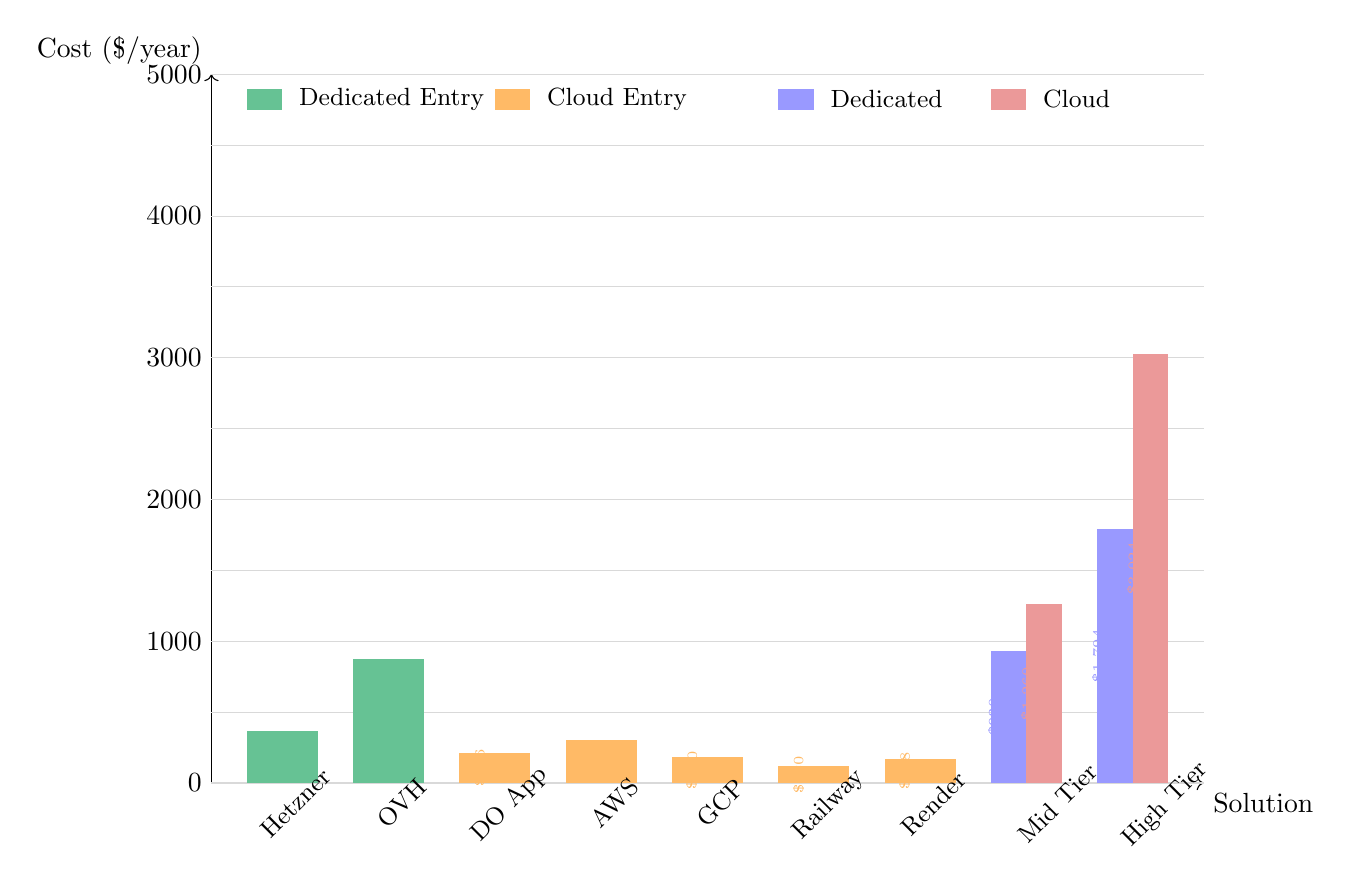
\begin{tikzpicture}[scale=0.9]
    % Y-axis
    \draw[->] (0,0) -- (0,10) node[anchor=south east] {Cost (\$/year)};
    % X-axis
    \draw[->] (0,0) -- (14,0) node[anchor=north west] {Solution};
    
    % Grid
    \foreach \y in {0,1,...,10}
        \draw[gray!30] (0,\y) -- (14,\y);
    
    % Y-axis labels (0 to 5000)
    \foreach \y/\ylabel in {0/0, 2/1000, 4/2000, 6/3000, 8/4000, 10/5000}
        \node[anchor=east] at (0,\y) {\ylabel};
    
    % Bars - Entry tier
    \fill[green!60] (0.5,0) rectangle (1.5,0.73) node[pos=.5, rotate=90, anchor=south] {\tiny \$366};
    \node[anchor=north, rotate=45] at (1,-0.1) {\small Hetzner};
    
    \fill[green!60] (2,0) rectangle (3,1.75) node[pos=.5, rotate=90, anchor=south] {\tiny \$876};
    \node[anchor=north, rotate=45] at (2.5,-0.1) {\small OVH};
    
    \fill[orange!60] (3.5,0) rectangle (4.5,0.43) node[pos=.5, rotate=90, anchor=south] {\tiny \$216};
    \node[anchor=north, rotate=45] at (4,-0.1) {\small DO App};
    
    \fill[orange!60] (5,0) rectangle (6,0.6) node[pos=.5, rotate=90, anchor=south] {\tiny \$300};
    \node[anchor=north, rotate=45] at (5.5,-0.1) {\small AWS};
    
    \fill[orange!60] (6.5,0) rectangle (7.5,0.36) node[pos=.5, rotate=90, anchor=south] {\tiny \$180};
    \node[anchor=north, rotate=45] at (7,-0.1) {\small GCP};
    
    \fill[orange!60] (8,0) rectangle (9,0.24) node[pos=.5, rotate=90, anchor=south] {\tiny \$120};
    \node[anchor=north, rotate=45] at (8.5,-0.1) {\small Railway};
    
    \fill[orange!60] (9.5,0) rectangle (10.5,0.34) node[pos=.5, rotate=90, anchor=south] {\tiny \$168};
    \node[anchor=north, rotate=45] at (10,-0.1) {\small Render};
    
    % Mid tier comparison
    \fill[blue!40] (11,0) rectangle (11.5,1.86) node[pos=.5, rotate=90, anchor=south] {\tiny \$930};
    \fill[red!40] (11.5,0) rectangle (12,2.52) node[pos=.5, rotate=90, anchor=south] {\tiny \$1,260};
    \node[anchor=north, rotate=45] at (11.75,-0.1) {\small Mid Tier};
    
    % High tier comparison
    \fill[blue!40] (12.5,0) rectangle (13,3.59) node[pos=.5, rotate=90, anchor=south] {\tiny \$1,794};
    \fill[red!40] (13,0) rectangle (13.5,6.05) node[pos=.5, rotate=90, anchor=south] {\tiny \$3,024};
    \node[anchor=north, rotate=45] at (13.25,-0.1) {\small High Tier};
    
    % Legend
    \fill[green!60] (0.5,9.5) rectangle (1,9.8);
    \node[anchor=west] at (1.1,9.65) {\small Dedicated Entry};
    
    \fill[orange!60] (4,9.5) rectangle (4.5,9.8);
    \node[anchor=west] at (4.6,9.65) {\small Cloud Entry};
    
    \fill[blue!40] (8,9.5) rectangle (8.5,9.8);
    \node[anchor=west] at (8.6,9.65) {\small Dedicated};
    
    \fill[red!40] (11,9.5) rectangle (11.5,9.8);
    \node[anchor=west] at (11.6,9.65) {\small Cloud};
\end{tikzpicture}
\caption{Annual Cost Comparison Across Platforms}
\end{figure}

\textbf{Key Cost Insights:}
\begin{itemize}
    \item Railway/Render offer the lowest entry point (\$60-\$384/year) for MVP
    \item Dedicated servers become cost-effective at mid-tier (saves 25-40\%)
    \item AWS/Azure/GCP have higher baseline costs but better scaling economics
    \item Hidden costs:  bandwidth overages on AWS (\$0.09/GB), egress fees
    \item DigitalOcean offers predictable pricing with no bandwidth surprises
\end{itemize}

\newpage

% Performance Comparison
\section{Performance Comparison}

\subsection{CPU Performance for PDF Generation}

Your ReportLab + Matplotlib workload is single-threaded and CPU-intensive.  Benchmarks based on Geekbench scores and real-world FastAPI testing: 

\begin{table}[H]
\centering
\caption{PDF Generation Performance Estimates (10-page report with 3 charts)}
\begin{tabularx}{\textwidth}{|l|l|X|l|l|}
\hline
\rowcolor{headerblue}
\textcolor{white}{\textbf{Platform}} & \textcolor{white}{\textbf{CPU Type}} & \textcolor{white}{\textbf{Single-Core Score}} & \textcolor{white}{\textbf{Render Time}} & \textcolor{white}{\textbf{Rating}} \\
\hline
\textbf{Hetzner Ryzen 5 3600} & Physical & 1250 & 2.1s & \pro\pro\pro \\
\hline
\textbf{OVH EPYC 7351P} & Physical & 950 & 2.8s & \pro\pro \\
\hline
\textbf{AWS t3.medium} & Burstable & 750 & 3.5s* & \pro\pro \\
\hline
\textbf{GCP e2-standard-2} & Shared & 680 & 3.9s & \pro \\
\hline
\textbf{DO Premium 4GB} & Shared & 720 & 3.7s & \pro\pro \\
\hline
\textbf{Azure B2s} & Burstable & 640 & 4.1s* & \pro \\
\hline
\textbf{Railway Starter} & Shared & 550 & 4.8s & \pro \\
\hline
\textbf{Render Standard} & Shared & 580 & 4.5s & \pro \\
\hline
\textbf{Heroku Standard-1X} & Shared & 520 & 5.1s & \neutral \\
\hline
\end{tabularx}
\end{table}

\textit{* Burstable instances may throttle after sustained load (CPU credit depletion)}

\textbf{Performance Optimization Strategies:}
\begin{enumerate}
    \item \textbf{Async Task Queue: } Implement Celery + Redis to offload PDF generation
    \item \textbf{Caching:} Cache PDFs with hash of assessment answers (avoid regeneration)
    \item \textbf{Lazy Loading:} Generate PDFs on-demand, not during assessment submission
    \item \textbf{Dedicated Workers:} Separate worker instances for PDF generation (cloud)
    \item \textbf{Serverless Offload:} Use AWS Lambda for PDF generation (cold start penalty)
\end{enumerate}

\subsection{Database I/O Performance}

SQLite performs well for <100 concurrent connections, but PostgreSQL is required for production:

\begin{table}[H]
\centering
\caption{Database Performance Comparison (IOPS \& Query Latency)}
\begin{tabularx}{\textwidth}{|l|l|X|l|l|}
\hline
\rowcolor{headerblue}
\textcolor{white}{\textbf{Database Service}} & \textcolor{white}{\textbf{Storage}} & \textcolor{white}{\textbf{Max IOPS}} & \textcolor{white}{\textbf{Latency}} & \textcolor{white}{\textbf{Connections}} \\
\hline
\textbf{Self-managed NVMe} & NVMe SSD & 100,000+ & <1ms & 100+ \\
\hline
\textbf{AWS RDS (gp3)} & EBS gp3 & 16,000 & 1-3ms & 87 (t3.micro) \\
\hline
\textbf{GCP Cloud SQL (SSD)} & Persistent SSD & 15,000 & 2-4ms & 25 (micro) \\
\hline
\textbf{Azure Database} & Premium SSD & 12,000 & 2-5ms & 50 (Basic) \\
\hline
\textbf{DO Managed DB} & SSD & 8,000 & 3-6ms & 25 (1GB) \\
\hline
\textbf{Railway Postgres} & SSD & 5,000 & 5-10ms & 20 (Starter) \\
\hline
\textbf{Render Postgres} & SSD & 4,000 & 5-12ms & 22 (Starter) \\
\hline
\end{tabularx}
\end{table}

\textbf{For Your Application:}
\begin{itemize}
    \item Expected read/write ratio: 70/30 (assessments are read-heavy)
    \item Connection pooling recommended:  SQLAlchemy \texttt{pool\_size=20, max\_overflow=10}
    \item Index optimization: Add indexes on \texttt{user\_id}, \texttt{assessment\_id}, \texttt{created\_at}
    \item Query optimization: Use SQLAlchemy \texttt{joinedload()} for relationships
\end{itemize}

\subsection{Network Latency \& Throughput}

\begin{table}[H]
\centering
\caption{Global Latency Comparison (from Middle East/North Africa)}
\begin{tabularx}{\textwidth}{|l|X|l|l|}
\hline
\rowcolor{headerblue}
\textcolor{white}{\textbf{Provider}} & \textcolor{white}{\textbf{Nearest Region}} & \textcolor{white}{\textbf{Avg Latency}} & \textcolor{white}{\textbf{Bandwidth}} \\
\hline
\textbf{Hetzner} & Germany (Falkenstein) & 80-120ms & 1 Gbps \\
\hline
\textbf{OVH} & France (Gravelines) & 70-110ms & 1 Gbps \\
\hline
\textbf{AWS} & Bahrain (me-south-1) & 20-50ms & Up to 5 Gbps \\
\hline
\textbf{GCP} & Tel Aviv (me-west1) & 30-60ms & Up to 16 Gbps \\
\hline
\textbf{Azure} & UAE (uaenorth) & 15-40ms & Up to 15 Gbps \\
\hline
\textbf{DigitalOcean} & Germany (Frankfurt) & 80-120ms & 5 Tbps \\
\hline
\end{tabularx}
\end{table}

\textbf{Recommendation for Arabic/MENA Users:}
\begin{itemize}
    \item \textbf{Best latency:} AWS Bahrain, Azure UAE, or GCP Tel Aviv
    \item \textbf{Cost-effective:} Hetzner Germany + CloudFlare CDN (caching)
    \item \textbf{Hybrid: } Backend in Europe, CDN for static assets (React app)
\end{itemize}

\subsection{Static Asset Delivery Speed}

React/Vite builds produce highly optimized bundles.  CDN performance comparison:

\begin{table}[H]
\centering
\caption{CDN Performance for React Static Assets}
\begin{tabularx}{\textwidth}{|l|l|X|l|}
\hline
\rowcolor{headerblue}
\textcolor{white}{\textbf{CDN}} & \textcolor{white}{\textbf{Edge Locations}} & \textcolor{white}{\textbf{TTFB (Global Avg)}} & \textcolor{white}{\textbf{Cache Hit Ratio}} \\
\hline
\textbf{CloudFlare} & 300+ & 15-30ms & 95\%+ \\
\hline
\textbf{AWS CloudFront} & 450+ & 20-40ms & 90\%+ \\
\hline
\textbf{Vercel Edge} & 100+ & 25-45ms & 92\%+ \\
\hline
\textbf{Bunny CDN} & 100+ & 30-50ms & 88\%+ \\
\hline
\textbf{Self-hosted Nginx} & 1 & 80-200ms & 70\% \\
\hline
\end{tabularx}
\end{table}

\newpage

% Operational Complexity
\section{Operational Complexity}

\subsection{Setup Time Comparison}

\begin{table}[H]
\centering
\caption{Time-to-Production Estimates}
\begin{tabularx}{\textwidth}{|l|X|l|l|}
\hline
\rowcolor{headerblue}
\textcolor{white}{\textbf{Platform}} & \textcolor{white}{\textbf{Setup Steps}} & \textcolor{white}{\textbf{Time}} & \textcolor{white}{\textbf{Complexity}} \\
\hline
\textbf{Railway} & Connect GitHub → Auto-deploy & 15-30 min & \textcolor{green}{Low} \\
\hline
\textbf{Render} & Connect GitHub → Configure build & 30-60 min & \textcolor{green}{Low} \\
\hline
\textbf{Heroku} & Git push + config vars & 1-2 hours & \textcolor{green}{Low} \\
\hline
\textbf{DO App Platform} & GitHub integration + database & 1-2 hours & \textcolor{orange}{Medium} \\
\hline
\textbf{AWS Lightsail} & Manual server setup + Nginx & 3-5 hours & \textcolor{orange}{Medium} \\
\hline
\textbf{AWS EC2 + RDS} & VPC, security groups, load balancer & 5-8 hours & \textcolor{red}{High} \\
\hline
\textbf{Dedicated Server} & OS install, Nginx, systemd, SSL & 4-8 hours & \textcolor{red}{High} \\
\hline
\textbf{Kubernetes (GKE/EKS)} & Cluster setup, manifests, ingress & 8-16 hours & \textcolor{red}{Very High} \\
\hline
\end{tabularx}
\end{table}

\subsection{Ongoing Maintenance Requirements}

\begin{table}[H]
\centering
\caption{Monthly Maintenance Hours (Estimate)}
\begin{tabularx}{\textwidth}{|l|X|l|l|}
\hline
\rowcolor{headerblue}
\textcolor{white}{\textbf{Task}} & \textcolor{white}{\textbf{Dedicated Server}} & \textcolor{white}{\textbf{Managed Cloud}} & \textcolor{white}{\textbf{Savings}} \\
\hline
\textbf{OS Updates} & 2-3 hours/month & 0 hours (automatic) & 100\% \\
\hline
\textbf{Security Patches} & 1-2 hours/month & 0 hours (automatic) & 100\% \\
\hline
\textbf{Database Backups} & 1 hour setup + monitoring & 0 hours (automatic) & 100\% \\
\hline
\textbf{SSL Renewal} & 30 min (Let's Encrypt) & 0 hours (automatic) & 100\% \\
\hline
\textbf{Monitoring Setup} & 2-4 hours initial & Built-in dashboards & 80\% \\
\hline
\textbf{Log Management} & 1-2 hours/month & Built-in (limited) & 50\% \\
\hline
\textbf{Scaling Adjustments} & 2-4 hours (manual) & 5 min (UI/API) & 95\% \\
\hline
\rowcolor{lightgray}
\textbf{Total Monthly} & \textbf{8-15 hours} & \textbf{1-2 hours} & \textbf{85-90\%} \\
\hline
\end{tabularx}
\end{table}

\textbf{DevOps Skill Requirements:}

\begin{itemize}
    \item \textbf{Dedicated Server: } Linux administration, Nginx/Apache, systemd, firewall (iptables/ufw), SSH hardening, backup scripts, monitoring tools (Prometheus/Grafana)
    \item \textbf{Managed Cloud:} Environment variables, CI/CD basics, cloud console navigation, database connection strings
\end{itemize}

\newpage

% Reliability & SLA
\section{Reliability \& Service Level Agreements}

\subsection{Uptime Guarantees}

\begin{table}[H]
\centering
\caption{SLA Comparison Across Platforms}
\begin{tabularx}{\textwidth}{|l|l|X|l|}
\hline
\rowcolor{headerblue}
\textcolor{white}{\textbf{Provider}} & \textcolor{white}{\textbf{SLA}} & \textcolor{white}{\textbf{Downtime/Year}} & \textcolor{white}{\textbf{Credits}} \\
\hline
\textbf{AWS} & 99.99\% & 52.56 minutes & Yes \\
\hline
\textbf{Google Cloud} & 99.95\% & 4.38 hours & Yes \\
\hline
\textbf{Azure} & 99.95\% & 4.38 hours & Yes \\
\hline
\textbf{DigitalOcean} & 99.99\% & 52.56 minutes & Yes \\
\hline
\textbf{Railway} & 99.9\% (est.) & 8.76 hours & No formal SLA \\
\hline
\textbf{Render} & 99.9\% (est.) & 8.76 hours & No formal SLA \\
\hline
\textbf{Heroku} & 99.95\% & 4.38 hours & Limited \\
\hline
\textbf{Hetzner} & 99.0\% & 3.65 days & No \\
\hline
\textbf{OVH} & 99.9\% & 8.76 hours & Limited \\
\hline
\end{tabularx}
\end{table}

\subsection{Support Response Times}

\begin{table}[H]
\centering
\caption{Support Tier Comparison}
\begin{tabularx}{\textwidth}{|l|X|l|l|}
\hline
\rowcolor{headerblue}
\textcolor{white}{\textbf{Provider}} & \textcolor{white}{\textbf{Support Channels}} & \textcolor{white}{\textbf{Response Time}} & \textcolor{white}{\textbf{Cost}} \\
\hline
\textbf{AWS} & Email, phone, chat & 1-24 hours & \$29-\$15K/mo \\
\hline
\textbf{Google Cloud} & Email, phone, chat & 1-24 hours & \$29-\$12.5K/mo \\
\hline
\textbf{Azure} & Email, phone, chat & 1-24 hours & \$29-\$1K/mo \\
\hline
\textbf{DigitalOcean} & Ticket, chat & 1-8 hours & Included \\
\hline
\textbf{Railway} & Discord, email & Community-driven & Included \\
\hline
\textbf{Render} & Email, chat & 4-24 hours & Included \\
\hline
\textbf{Heroku} & Email, ticket & 2-24 hours & \$0-\$1K/mo \\
\hline
\textbf{Hetzner} & Email, ticket & 12-48 hours & Included \\
\hline
\textbf{OVH} & Ticket, phone & 4-24 hours & Included \\
\hline
\end{tabularx}
\end{table}

\newpage

% Decision Framework
\section{Decision Framework \& Recommendations}

\subsection{Use Case-Based Recommendations}

\begin{table}[H]
\centering
\caption{Recommended Solutions by Phase}
\begin{tabularx}{\textwidth}{|l|X|X|l|}
\hline
\rowcolor{headerblue}
\textcolor{white}{\textbf{Phase}} & \textcolor{white}{\textbf{Recommended Solution}} & \textcolor{white}{\textbf{Rationale}} & \textcolor{white}{\textbf{Cost}} \\
\hline
\textbf{MVP} & Railway Hobby or & Fast deployment, minimal DevOps, & \$5-\$50/mo \\
\textbf{< 1K users} & Render Starter & usage-based pricing, easy scaling & \\
\hline
\textbf{Growth} & DigitalOcean Droplet & Predictable costs, good performance, & \$84-\$150/mo \\
\textbf{1K-10K} & + Managed PostgreSQL & balance of control \& simplicity & \\
\hline
\textbf{Scale} & AWS/GCP with & Auto-scaling, global reach, & \$300-\$800/mo \\
\textbf{> 10K users} & auto-scaling + RDS & enterprise features & \\
\hline
\end{tabularx}
\end{table}

\subsection{Decision Tree}

\begin{figure}[H]
\centering
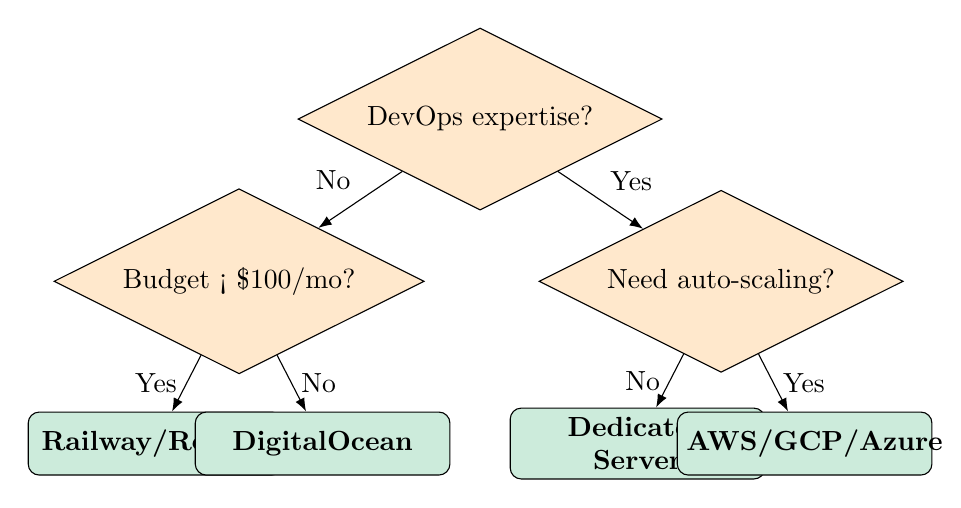
\begin{tikzpicture}[
    node distance=1.5cm,
    decision/.style={diamond, draw, fill=orange!20, text width=4cm, text centered, inner sep=0pt, aspect=2},
    block/.style={rectangle, draw, fill=blue!20, text width=3.5cm, text centered, rounded corners, minimum height=1cm},
    result/.style={rectangle, draw, fill=green!20, text width=3cm, text centered, rounded corners, minimum height=0.8cm},
    line/.style={draw, -Latex}
]

\node [decision] (start) {DevOps expertise? };
\node [decision, below left of=start, yshift=-1cm, xshift=-2cm] (budget) {Budget < \$100/mo?};
\node [decision, below right of=start, yshift=-1cm, xshift=2cm] (scale) {Need auto-scaling?};

\node [result, below left of=budget, yshift=-1cm] (railway) {\textbf{Railway/Render}};
\node [result, below right of=budget, yshift=-1cm] (do) {\textbf{DigitalOcean}};
\node [result, below left of=scale, yshift=-1cm] (dedicated) {\textbf{Dedicated Server}};
\node [result, below right of=scale, yshift=-1cm] (cloud) {\textbf{AWS/GCP/Azure}};

\path [line] (start) -- node [above left] {No} (budget);
\path [line] (start) -- node [above right] {Yes} (scale);
\path [line] (budget) -- node [left] {Yes} (railway);
\path [line] (budget) -- node [right] {No} (do);
\path [line] (scale) -- node [left] {No} (dedicated);
\path [line] (scale) -- node [right] {Yes} (cloud);

\end{tikzpicture}
\caption{Hosting Decision Tree}
\end{figure}

\subsection{Deal Breakers \& Critical Factors}

\begin{table}[H]
\centering
\caption{When to Choose Each Option}
\begin{tabularx}{\textwidth}{|l|X|X|}
\hline
\rowcolor{headerblue}
\textcolor{white}{\textbf{Factor}} & \textcolor{white}{\textbf{Choose Dedicated}} & \textcolor{white}{\textbf{Choose Cloud}} \\
\hline
\textbf{Budget} & >6 months, predictable load & Variable load, pay-as-you-go \\
\hline
\textbf{Traffic} & Steady, predictable & Spiky, seasonal \\
\hline
\textbf{Team Size} & Have DevOps engineer & Small team, no DevOps \\
\hline
\textbf{Time-to-Market} & Can wait 1-2 weeks & Need deployment this week \\
\hline
\textbf{Scaling} & Vertical scaling sufficient & Need horizontal scaling \\
\hline
\textbf{Compliance} & Full control required & Managed compliance OK \\
\hline
\textbf{Performance} & CPU-intensive workloads & I/O or network-intensive \\
\hline
\end{tabularx}
\end{table}

\newpage

% Actionable Next Steps
\section{Actionable Next Steps}

\subsection{Phase 1: MVP Launch (Weeks 1-4)}

\textbf{Recommended:  Railway Hobby Plan (\$5/month + usage)}

\begin{enumerate}
    \item \textbf{Week 1: Setup \& Migration}
    \begin{itemize}
        \item Create Railway account, connect GitHub repository
        \item Configure environment variables (database URL, secrets)
        \item Migrate SQLite to PostgreSQL using Alembic
        \item Test database migration with sample data
    \end{itemize}
    
    \item \textbf{Week 2: Deployment \& Testing}
    \begin{itemize}
        \item Deploy FastAPI backend to Railway
        \item Deploy React frontend to Vercel/Netlify (free tier)
        \item Configure CORS for production domains
        \item Set up SendGrid for email delivery (free 100/day)
    \end{itemize}
    
    \item \textbf{Week 3: Optimization}
    \begin{itemize}
        \item Implement Redis caching for assessment data
        \item Set up background task queue for PDF generation
        \item Configure CloudFlare CDN for static assets
        \item Add monitoring with Railway metrics
    \end{itemize}
    
    \item \textbf{Week 4: Launch \& Monitor}
    \begin{itemize}
        \item Perform load testing with expected user volume
        \item Set up UptimeRobot for availability monitoring
        \item Configure automated backups (Railway built-in)
        \item Launch to initial users
    \end{itemize}
\end{enumerate}

\textbf{Expected Monthly Cost: } \$20-\$50

\subsection{Phase 2: Growth (Months 2-6)}

\textbf{Recommended: DigitalOcean Droplet + Managed PostgreSQL}

\begin{enumerate}
    \item \textbf{Migration Planning}
    \begin{itemize}
        \item Containerize application with Docker
        \item Set up CI/CD pipeline (GitHub Actions)
        \item Plan database migration strategy
        \item Estimate resource requirements
    \end{itemize}
    
    \item \textbf{Infrastructure Setup}
    \begin{itemize}
        \item Provision 4GB DigitalOcean Droplet (\$24/mo)
        \item Set up managed PostgreSQL 4GB (\$60/mo)
        \item Configure Nginx reverse proxy with SSL
        \item Implement automated backup strategy
    \end{itemize}
    
    \item \textbf{Performance Optimization}
    \begin{itemize}
        \item Implement connection pooling (SQLAlchemy)
        \item Add database indexes for common queries
        \item Set up Redis for caching (DigitalOcean managed)
        \item Optimize PDF generation with worker processes
    \end{itemize}
    
    \item \textbf{Monitoring \& Alerting}
    \begin{itemize}
        \item Configure DigitalOcean monitoring
        \item Set up log aggregation
        \item Create performance dashboards
        \item Implement error tracking (Sentry free tier)
    \end{itemize}
\end{enumerate}

\textbf{Expected Monthly Cost:} \$90-\$150

\subsection{Phase 3: Scale (Months 6+)}

\textbf{Recommended: AWS Auto-scaling + RDS}

\begin{enumerate}
    \item \textbf{Architecture Redesign}
    \begin{itemize}
        \item Split frontend/backend deployment
        \item Implement microservices for PDF generation
        \item Set up load balancer (AWS ALB)
        \item Configure auto-scaling groups
    \end{itemize}
    
    \item \textbf{Database Optimization}
    \begin{itemize}
        \item Migrate to AWS RDS with read replicas
        \item Implement database connection pooling
        \item Set up automated backups with point-in-time recovery
        \item Configure performance insights
    \end{itemize}
    
    \item \textbf{Global Distribution}
    \begin{itemize}
        \item Deploy to multiple AWS regions
        \item Configure CloudFront CDN
        \item Implement edge caching strategies
        \item Set up global load balancing
    \end{itemize}
    
    \item \textbf{Enterprise Features}
    \begin{itemize}
        \item Implement comprehensive monitoring (DataDog)
        \item Set up disaster recovery procedures
        \item Configure compliance controls (SOC 2)
        \item Implement advanced security measures
    \end{itemize}
\end{enumerate}

\textbf{Expected Monthly Cost: } \$300-\$800

\newpage

% Appendix
\section{Appendix}

\subsection{Resource Links}

\textbf{Cloud Platforms: }
\begin{itemize}
    \item Railway: \url{https://railway.app/pricing}
    \item Render:  \url{https://render.com/pricing}
    \item DigitalOcean: \url{https://www.digitalocean.com/pricing}
    \item AWS: \url{https://aws.amazon.com/pricing/}
    \item Google Cloud: \url{https://cloud.google.com/pricing}
\end{itemize}

\textbf{Dedicated Servers:}
\begin{itemize}
    \item Hetzner: \url{https://www.hetzner.com/dedicated-rootserver}
    \item OVH: \url{https://www.ovhcloud.com/en/bare-metal/}
\end{itemize}

\textbf{Tools \& Services:}
\begin{itemize}
    \item SendGrid (Email): \url{https://sendgrid.com/pricing/}
    \item CloudFlare (CDN): \url{https://www.cloudflare.com/plans/}
    \item UptimeRobot (Monitoring): \url{https://uptimerobot.com/pricing/}
\end{itemize}

\subsection{Cost Calculator Spreadsheet}

A detailed Excel/Google Sheets calculator is available with this report that allows you to:
\begin{itemize}
    \item Input your expected user volume
    \item Estimate bandwidth and storage requirements
    \item Compare total cost of ownership across platforms
    \item Model different growth scenarios
    \item Calculate break-even points between options
\end{itemize}

\subsection{Glossary}

\begin{description}
    \item[vCPU] Virtual Central Processing Unit - A portion of a physical CPU allocated to a virtual machine
    \item[IOPS] Input/Output Operations Per Second - Measure of storage performance
    \item[TCO] Total Cost of Ownership - All costs associated with a solution over time
    \item[SLA] Service Level Agreement - Guaranteed uptime and performance metrics
    \item[RTO] Recovery Time Objective - Maximum acceptable downtime
    \item[RPO] Recovery Point Objective - Maximum acceptable data loss
    \item[CDN] Content Delivery Network - Distributed system for delivering content globally
\end{description}

\newpage

% Conclusion
\section{Conclusion}

Based on comprehensive analysis of technical requirements, cost projections, and operational complexity, the following recommendations are made for your career assessment platform:

\subsection{Summary of Recommendations}

\begin{enumerate}
    \item \textbf{Immediate Action (MVP Phase):} Deploy on Railway or Render for fastest time-to-market with minimal costs (\$5-\$50/month). This allows you to validate your product-market fit without significant infrastructure investment. 
    
    \item \textbf{Growth Strategy:} Migrate to DigitalOcean when you reach 1,000+ active users. This provides better performance-per-dollar while maintaining operational simplicity through managed services.
    
    \item \textbf{Scale Approach:} For 10K+ users, leverage AWS/GCP auto-scaling infrastructure with managed databases to ensure global availability and performance.
    
    \item \textbf{CPU Optimization:} Given your PDF generation workload, implement async task queues (Celery + Redis) regardless of chosen platform to prevent blocking API requests.
    
    \item \textbf{Hybrid Architecture:} Consider hosting the backend in Europe (cost-effective) while using CloudFlare CDN for global content delivery and reduced latency for MENA users.
\end{enumerate}

\subsection{Final Recommendation}

For the CaRhythm platform in January 2026, we recommend:

\textbf{Phase 1 (Immediate):} Railway Hobby Plan (\$20-\$50/month)
\begin{itemize}
    \item Fastest deployment (15-30 minutes)
    \item Zero DevOps overhead
    \item PostgreSQL included
    \item Usage-based scaling
\end{itemize}

\textbf{Phase 2 (At 1K users):} DigitalOcean Droplet + Managed DB (\$90-\$150/month)
\begin{itemize}
    \item Predictable costs
    \item Better CPU performance for PDF generation
    \item Full control with managed database
    \item Docker-based deployment
\end{itemize}

\textbf{Phase 3 (At 10K+ users):} AWS/GCP with auto-scaling (\$300-\$800/month)
\begin{itemize}
    \item Global distribution
    \item Automatic horizontal scaling
    \item Enterprise-grade reliability
    \item Advanced monitoring and analytics
\end{itemize}

\vspace{1cm}

\noindent This strategic approach minimizes initial investment while providing clear migration paths as your platform grows. The total cost of ownership over 24 months is estimated at \$720-\$2,400 for the MVP phase, with ROI improving as user base expands.

\vspace{0.5cm}

\noindent\textbf{Next Step:} Begin with Railway deployment to validate market fit, then reassess infrastructure needs based on actual usage patterns and growth metrics.

\end{document}